\chapter{Descripción del problema}

En este capítulo se planteará en detalle el problema a resolver. Tras esto, se comentarán soluciones previas propuestas al problema, y se describirán los objetivos que se esperan alcanzar con el desarrollo del trabajo. 

\section{Definición del problema}

El problema a resolver es el diseño de un agente físico (un robot) capaz de navegar desde una posición inicial hasta una posición final (conocidas sus coordenadas) en un entorno de interior del que no se tiene conocimiento previo (como puede ser el interior de una casa) de forma eficiente. Este problema se encuadra en el campo de la navegación automática, concretamente en el de la \textbf{navegación a meta} (\textit{Point Goal Navigation}) \textbf{sin exploración previa} del entorno \cite{DBLP:journals/corr/abs-1807-06757}.

Para lograr esto, es necesario entrenar al agente en un entorno controlado para que aprenda a navegar de forma autónoma en interiores desconocidos, usando alguna técnica de aprendizaje por refuerzo. Además. se busca que el agente sea capaz de navegar \textbf{sin exploración previa} (como se ha mencionado anteriormente), buscando un sistema reactivo frente a uno basado en exploración-navegación.

El agente físico cuenta con las siguientes características a tener en cuenta:
\begin{itemize}
	\item \textbf{Movimiento:} El agente es terrestre (se desplaza con ruedas sobre el suelo), pudiendo moverse hacia adelante y rotar sobre si mismo. El agente no es capaz de realizar movimientos ortogonales.
	\item \textbf{Sensores:} El agente cuenta con dos sensores para recibir información del entorno: una \textbf{cámara de profundidad} para observar el espacio frente al robot y un \textbf{GPS}, indicando la distancia y ángulo hasta la meta.
\end{itemize}

\section{Antecedentes}

La navegación autónoma de robots en interiores es un campo de gran interés tanto para la investigación como para la industria, existiendo gran cantidad de grupos dedicados a la propuesta y desarrollo de agentes capaces de resolver estos problemas de forma eficaz.

Algunos ejemplos de este interés \textit{Habitat Challenge}, un desafío anual organizado por  \textit{Facebook AI Research} (el grupo de investigación de inteligencia artificial de Facebook) parte de la \textit{Conference on Computer Vision and Pattern Recognition (CVPR)} en el que se buscan los mejores algoritmos para resolver problemas de \textbf{navegación autónoma a metas} \cite{habitat2020sim2real} (aunque también incluye problemas de \textbf{navegación autónoma a objetos} \cite{batra2020objectnav}) aplicados a agentes físicos en entornos de interiores. Algunas de las mejores propuestas de estos últimos años han sido:
 
\begin{itemize}
	\item \textbf{Devendra Singh Chaplot \textit{et al.} (2019)} \cite{DBLP:journals/corr/abs-2004-05155}: Se propone un nuevo algoritmo, \textit{Active Neural SLAM}, que combina las capacidades de planificadores de ruta clásicos como SLAM con la capacidad del aprendizaje por refuerzo profundo para generar políticas de acciones locales y globales. Esta propuesta obtuvo el primer puesto del \textit{Habitat Challenge 2019}.
	\item \textbf{Santhosh K. Ramakrishnan \textit{et al.} (2020)} \cite{DBLP:journals/corr/abs-2008-09285}: Se propone un sistema de navegación entrenado con aprendizaje por refuerzo que, a partir de sus observaciones a través de una cámara RGB, es capaz de inferir la posición de los objetos más allá de su ángulo de visión para mejorar su rendimiento a la hora de generar un mapa de su entorno. Esta propuesta alcanzó el primer puesto del \textit{Habitat Challenge 2020}.
	 \item \textbf{Samyak Datta \textit{et al.} (2020)} \cite{DBLP:journals/corr/abs-2009-03231}: Se propone un sistema de navegación entrenado con aprendizaje por refuerzo (\textit{PPO}) que tiene en cuenta el ruido existente en entornos reales (problemas durante la actuación, desviaciones entre la posición real y estimada...) haciendo esfuerzo para corregirlo. Esta propuesta alcanzó el segundo puesto del \textit{Habitat Challenge 2020}.
	 \item \textbf{Ruslan Partsey (2021)} \cite{Partsey2021}: Se desarrolla un agente que usa técnicas de odometría (usar datos de sensores de movimiento para estimar la posición real) visual con aprendizaje por refuerzo para conseguir una navegación eficiente en entornos con ruido. Esta propuesta alcanzó el primer puesto del \textit{Habitat Challenge 2021}.
\end{itemize}

Si bien todas las propuestas anteriores utilizan técnicas de aprendizaje por refuerzo, la gran mayoría de éstas utilizan enfoques basados en el mapeado y navegación de los entornos, frente a una propuesta puramente reactiva (sin mapa) como la de éste trabajo.

El antecedente más directo al trabajo descrito en esta memoria es la propuesta realizada por \textbf{Carlos Sampedro \textit{et al.} (2018)} \cite{Sampedro2018}, siendo éste trabajo una adaptación y continuación directa. El agente propuesto utiliza un método basado en campos de potenciales, entrenado con aprendizaje por refuerzo profundo para navegar un dron aéreo a través de entornos de interior, usando un conjunto de láseres (para percibir el entorno a su alrededor) y la posición relativa del propio dron respecto a la meta, con buenos resultados. Esta arquitectura se puede observar en la Figura \ref{fig:chap2-drone}.

\begin{figure}[h]
    \centering
    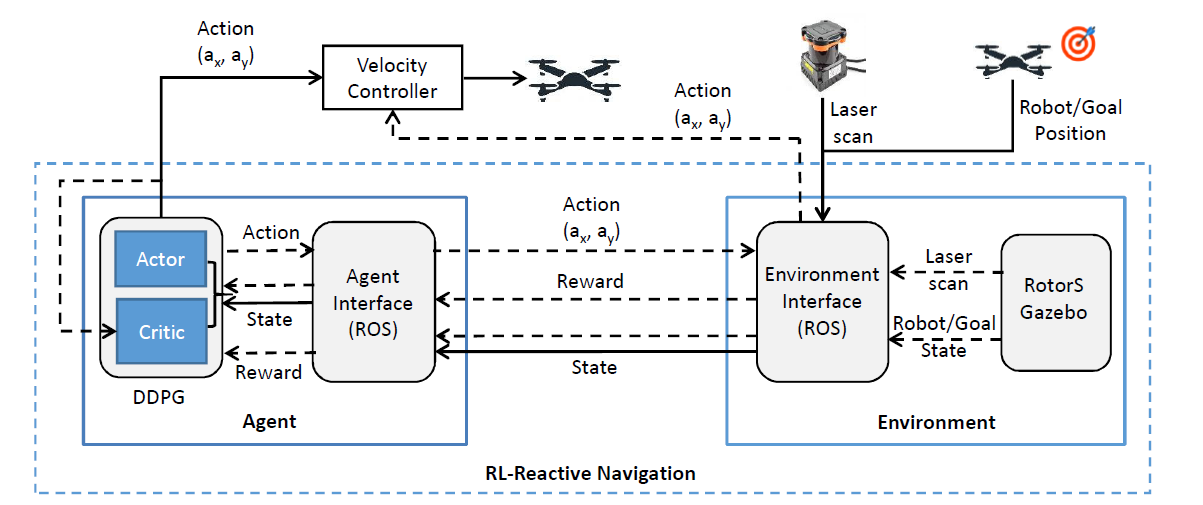
\includegraphics[width=\textwidth]{imagenes/cap2/drone-architecture.png}
    \caption{Arquitectura propuesta para el sistema de navegación reactivo original \cite{Sampedro2018}.}
    \label{fig:chap2-drone}
\end{figure}

Ahora bien, existen diferencias destacables entre la propuesta original y el trabajo descrito en esta memoria:

\begin{itemize}
	\item \textbf{Movimientos del agente:} La propuesta original utiliza como agente a un dron multirotor, capaz de navegar por el aire (aunque se mantiene a una altura constante) y de realizar movimiento omnidireccional. En cambio, el trabajo desarrollado utiliza un robot terrestre (susceptible a obstáculos en el suelo) incapaz de movimiento omnidireccional, siendo necesario el giro del agente para poder esquivar obstáculos y desplazarse.
	\item \textbf{Sensores del agente:} Mientras que la propuesta original utiliza un conjunto de láseres para percibir su entorno, el trabajo desarrollado propone un agente con una única cámara de profundidad frontal. Si bien el conjunto de láseres resulta más caro que una cámara de profundidad, también ofrece un ángulo de visión mayor de los obstáculos del entorno.
	\item \textbf{Complejidad del entorno:} La propuesta original entrena al agente en entornos de interior simples (contando con espacios simples con obstáculos dispersos), frente a los entornos usados por el trabajo desarrollado (siendo recreaciones del interior de domicilios, incluyendo topografías más complejas con cuartos y una mayor cantidad de obstáculos y ruido).
\end{itemize}

\section{Objetivos}

El principal objetivo de este trabajo es el estudio y aplicación de técnicas de aprendizaje por refuerzo profundo y navegación autónoma basada en campos de potenciales para el desarrollo de un agente capaz de navegar entornos de interior, evaluando su viabilidad y eficacia.

Para cumplir este objetivo, es necesario a su vez cumplir una serie de objetivos parciales:

\begin{itemize}
	\item Revisión de bibliografía para comprender plenamente las técnicas a usar durante el desarrollo.
	\item Búsqueda y evaluación de librerías y herramientas disponibles para el desarrollo del agente (incluyendo simuladores, entornos de trabajo...)
	\item Caracterización, formalización e implementación del agente y de posibles variaciones propuestas dentro del entorno elegido, para poder ser evaluado posteriormente.
	\item Realización de experimentos para estudiar el comportamiento del agente durante el entrenamiento y posteriormente al enfrentarse a problemas reales.
	\item Estudio y análisis de los resultados, realizando comparación con \textit{benchmarks} para extraer observaciones y conclusiones que permitan valorar la viabilidad y eficacia del agente propuesto.
\end{itemize}

Este trabajo además aborda un segundo objetivo, el estudio y uso del simulador \textit{Habitat Sim}, con el fin de evaluar su utilidad de cara a posteriores trabajos. Para esto, se plantean los siguientes objetivos parciales:

\begin{itemize}
	\item Revisión y estudio de documentación oficial y ejemplos ofrecidos por el simulador.
	\item Desarrollo del agente descrito previamente en el marco del simulador, usando las herramientas ofrecidas.
	\item Creación de documentación sobre el uso adecuado del simulador para facilitar trabajos posteriores.
	\item Evaluación de la idoneidad del simulador para la resolución de problemas de navegación autónoma.
\end{itemize}